%%%%%%%%%%%%%%%%%%%%%%%%%%%%%%%%%%%%
% Slide options
%%%%%%%%%%%%%%%%%%%%%%%%%%%%%%%%%%%%

% Option 1: Slides with solutions

\documentclass[slidestop,compress,mathserif]{beamer}
\newcommand{\soln}[1]{\textit{#1}}
\newcommand{\solnGr}[1]{#1}

\usepackage{todonotes}

% Option 2: Handouts without solutions

%\documentclass[11pt,containsverbatim,handout]{beamer}
%\usepackage{pgfpages}
%\pgfpagesuselayout{4 on 1}[letterpaper,landscape,border shrink=5mm]
%\newcommand{\soln}[1]{ }
%\newcommand{\solnGr}{ }

%%%%%%%%%%%%%%%%%%%%%%%%%%%%%%%%%%%%
% Style
%%%%%%%%%%%%%%%%%%%%%%%%%%%%%%%%%%%%

%%%%%%%%%%%%%%%%%%%%%%%%%%%%%%%%%%%%%%%%%%%%%%%%%%%%%%%%%%%%%%%%%%%%%%%%
% MA213/214 shared slide style
%
% "Calm & Cool" palette + content-type callout boxes.
% Overhauled (2026) from the original OpenIntro/metropolis style:
%   - all OpenIntro visual branding removed (logo, grid, colors)
%   - a low-key cool palette (see colors below)
%   - tcolorbox callout boxes so students recognize content types
% See common/README.md for the command cheat-sheet.
%%%%%%%%%%%%%%%%%%%%%%%%%%%%%%%%%%%%%%%%%%%%%%%%%%%%%%%%%%%%%%%%%%%%%%%%

\usetheme{metropolis}

%%%%%%%%%%%%%%%%
% Packages
%%%%%%%%%%%%%%%%

\usepackage{geometry}
\usepackage{graphicx}
\usepackage{amssymb}
\usepackage{epstopdf}
\usepackage{amsmath}  	% this permits text in eqnarray among other benefits
\usepackage{url}		% produces hyperlinks
\usepackage{hyperref}	% allows for color usage in tables
\usepackage[english]{babel}
\usepackage[latin1]{inputenc}
\usepackage{colortbl}	% allows for color usage in tables
\usepackage{multirow}	% allows for rows that span multiple rows in tables
\usepackage{color}		% this package has a variety of color options
\usepackage{pgf}
\usepackage{calc}
\usepackage{ulem}
\usepackage{multicol}
\usepackage{textcomp}
\usepackage{txfonts}
\usepackage{listings}
\usepackage{tikz}
\usepackage{array}
\usepackage{wasysym}
\usepackage{fancyvrb}
\usepackage{etoolbox}             % \ifstrempty for optional box subtitles
\usepackage[most]{tcolorbox}      % content-type callout boxes
\tcbuselibrary{listings}          % R-code block (\begin{rblock})
\usepackage{fontawesome5}         % box icons

%%%%%%%%%%%%%%%%
% Remove navigation symbols
%%%%%%%%%%%%%%%%

\setbeamertemplate{navigation symbols}{}

%%%%%%%%%%%%%%%%
% "Calm & Cool" palette
%%%%%%%%%%%%%%%%

% chrome / structure / body
\definecolor{ccSlate}{HTML}{2E3742}   % frametitle bar, structure, section pages (deep neutral slate)
\definecolor{ccInk}{HTML}{2B2B2B}     % body text
\definecolor{ccWash}{HTML}{FCF8F1}    % gentle warm title-slide background wash (complements the cool blues)

% example (blue)
\definecolor{ccBlue}{HTML}{2F6690}
\definecolor{ccBlueBg}{HTML}{EAF1F7}
% interactive activity / discussion (green)
\definecolor{ccGreen}{HTML}{4E8A6B}
\definecolor{ccGreenBg}{HTML}{E9F3EC}
% solution (purple)
\definecolor{ccPurple}{HTML}{6F5499}
\definecolor{ccPurpleBg}{HTML}{EFEAF6}
% worksheet / focused work (terracotta)
\definecolor{ccTerra}{HTML}{C2693E}
\definecolor{ccTerraBg}{HTML}{FAEDE4}
% formula / definition (neutral slate)
\definecolor{ccGray}{HTML}{5C6B7A}
\definecolor{ccGrayBg}{HTML}{EEF1F4}
% caution / common pitfall (brick red)
\definecolor{ccRed}{HTML}{B23A48}
\definecolor{ccRedBg}{HTML}{FAEAEC}
% key idea / takeaway (muted gold)
\definecolor{ccGold}{HTML}{9C7A28}
\definecolor{ccGoldBg}{HTML}{F7F1DF}
% learning goals / lesson outcomes (teal)
\definecolor{ccTeal}{HTML}{2C6E6B}
\definecolor{ccTealBg}{HTML}{E6F0EF}
% learning objectives (indigo)
\definecolor{ccIndigo}{HTML}{45507A}
\definecolor{ccIndigoBg}{HTML}{ECEEF4}
% R code / output (gray)
\definecolor{ccCode}{HTML}{5F5E5A}
\definecolor{ccCodeBg}{HTML}{F4F5F6}

% neutral grays kept from the original style
\definecolor{gray}{rgb}{0.5, 0.5, 0.5}
\definecolor{darkGray}{rgb}{0.3, 0.3, 0.3}
\definecolor{darkerGray}{rgb}{0.2, 0.2, 0.2}

% Backwards-compatible aliases: old OpenIntro color names now point at the
% new palette, so existing \textcolor{oiB}{...}, \hl{...}, etc. keep working.
\colorlet{oiB}{ccBlue}
\colorlet{oiG}{ccGreen}
\colorlet{hlblue}{ccBlue}
\colorlet{rubineRed}{ccRed}
\colorlet{irishGreen}{ccGreen}
\colorlet{lightGreen}{ccGreen}

%%%%%%%%%%%%%%%%
% Restyle metropolis with the Calm & Cool chrome
%%%%%%%%%%%%%%%%

\metroset{block=fill}

\setbeamercolor{normal text}{fg=ccInk, bg=white}
\setbeamercolor{structure}{fg=ccSlate}
\setbeamercolor{alerted text}{fg=ccBlue}
\setbeamercolor{example text}{fg=ccGreen}
\setbeamercolor{frametitle}{bg=ccSlate, fg=white}
\setbeamercolor{progress bar}{fg=ccBlue}
\setbeamercolor{title separator}{fg=ccBlue}
\setbeamercolor{title}{fg=ccSlate}
\setbeamercolor{subtitle}{fg=ccBlue}
\setbeamercolor{author}{fg=ccInk}
\setbeamercolor{institute}{fg=ccGray}
\setbeamercolor{date}{fg=ccGray}
\setbeamercolor{section title}{fg=ccSlate}
\setbeamercolor{standout}{fg=white, bg=ccSlate}

% Section pages sit on the same warm wash as the title slide. We keep
% metropolis's section-title styling and just paint a full-page ccWash
% background behind it (needs >=2 pdflatex passes for the current-page node).
\setbeamertemplate{section page}{%
  \begin{tikzpicture}[remember picture, overlay]
    \fill[ccWash] (current page.south west) rectangle (current page.north east);
  \end{tikzpicture}%
  \centering
  \begin{minipage}{22em}
    \raggedright
    \usebeamercolor[fg]{section title}%
    \usebeamerfont{section title}%
    \insertsectionhead\\[-1ex]
    \usebeamertemplate*{progress bar in section page}%
    \par
  \end{minipage}\par
  \vspace{\baselineskip}
}

%%%%%%%%%%%%%%%%
% Custom inline text commands (recolored to the palette)
%%%%%%%%%%%%%%%%

% degree
\newcommand{\degree}{\ensuremath{^\circ}}

% cite
\newcommand{\ct}[1]{
\vfill
{\tiny #1}}

\newcommand{\NamedNote}[2]{
\rule{2.5cm}{0.25pt} \\ \textit{\footnotesize{\textcolor{rubineRed}{#1:} \textcolor{darkerGray}{#2}}}}

% Note
\newcommand{\Note}[1]{
\rule{2.5cm}{0.25pt} \\ \textit{\footnotesize{\textcolor{rubineRed}{Note:} \textcolor{darkerGray}{#1}}}}

% Remember
\newcommand{\Remember}[1]{\textit{\scriptsize{\textcolor{ccTerra}{Remember:} #1}}}

% expected counts
\newcommand{\ex}[1]{\textit{\textcolor{ccBlue}{#1}}}

% red
\newcommand{\red}[1]{\textit{\textcolor{rubineRed}{#1}}}

% pink
\newcommand{\pink}[1]{\textit{\textcolor{rubineRed!90!white!50}{#1}}}

% green
\newcommand{\green}[1]{\textit{\textcolor{irishGreen}{#1}}}

% orange
\newcommand{\orange}[1]{\textit{\textcolor{ccTerra}{#1}}}

% links: webURL, webLink, appLink
\newcommand{\webURL}[1]{\urlstyle{same}{ \textit{\textcolor{darkGray}{\url{#1}}}}}
\newcommand{\webLink}[2]{\href{#1}{\textcolor{darkGray}{{#2}}}}
\newcommand{\appLink}[2]{\href{#1}{\textcolor{white}{{#2}}}}

% mail
\newcommand{\mail}[1]{\href{mailto:#1}{\textit{\textcolor{darkGray}{#1}}}}

% highlighting: hl, hlGr, mathhl
\newcommand{\hl}[1]{\textit{\textcolor{hlblue}{#1}}}
\newcommand{\hlGr}[1]{\textit{\textcolor{lightGreen}{#1}}}
\newcommand{\mathhl}[1]{\textcolor{hlblue}{\ensuremath{#1}}}

%%%%%%%%%%%%%%%%
% Structural helpers (unchanged from the original)
%%%%%%%%%%%%%%%%

% two col: two columns
\newenvironment{twocol}[4]{
\begin{columns}[c]
\column{#1\textwidth}
#3
\column{#2\textwidth}
#4
\end{columns}
}

% slot (for probability calculations)
\newenvironment{slot}[2]{
\begin{array}{c}
\underline{#1} \\
#2
\end{array}
}

% pr: left and right parentheses
\newcommand{\pr}[1]{
\left( #1 \right)
}

% cancel
\newcommand{\cancel}[1]{%
    \tikz[baseline=(tocancel.base)]{
        \node[inner sep=0pt,outer sep=0pt] (tocancel) {#1};
        \draw[red, line width=0.5mm] (tocancel.south west) -- (tocancel.north east);
    }%
}

% removepagenumbers
\newcommand{\removepagenumbers}{%
  \setbeamertemplate{footline}{}
}

% change margin
\newenvironment{changemargin}[2]{%
\begin{list}{}{%
\setlength{\topsep}{0pt}%
\setlength{\leftmargin}{#1}%
\setlength{\rightmargin}{#2}%
\setlength{\listparindent}{\parindent}%
\setlength{\itemindent}{\parindent}%
\setlength{\parsep}{\parskip}%
}%
\item}{\end{list}}

% footnote
\long\def\symbolfootnote[#1]#2{\begingroup%
\def\thefootnote{\fnsymbol{footnote}}\footnote[#1]{#2}\endgroup}

% commands from the book
\newenvironment{data}[1]{\texttt{#1}}{}
\newenvironment{var}[1]{\texttt{#1}}{}
\newenvironment{resp}[1]{\texttt{#1}}{}

%%%%%%%%%%%%%%%%
% Content-type callout boxes (tcolorbox)
%
% Each type has a colored title strip (icon + label) over a light fill.
% Color = content type; the label + icon reinforce it (so the cue does
% not rely on color alone).
%%%%%%%%%%%%%%%%

\tcbset{
  cccallout/.style 2 args={
    enhanced, breakable=false,
    colback=#2, colframe=#1, colbacktitle=#1, coltitle=white,
    fonttitle=\bfseries\footnotesize,
    boxrule=0.6pt, arc=2.5pt, outer arc=2.5pt,
    left=5pt, right=5pt, top=3pt, bottom=3pt, boxsep=2pt,
    toptitle=2pt, bottomtitle=2pt, lefttitle=5pt,
    before skip=5pt, after skip=5pt,
  },
}

% One-off / collection of examples (blue): \workedexample[subtitle]{body}.
% (Named \workedexample, not \example, because beamer defines \example.)
\newtcolorbox{examplebox}[1][]{cccallout={ccBlue}{ccBlueBg},
  title={\faIcon{lightbulb}~~Example\ifstrempty{#1}{}{ \textmd{---}\ #1}}}
\newcommand{\workedexample}[2][]{\begin{examplebox}[#1]#2\end{examplebox}}

% Running-example header (blue): \examplehead{name} at the top of each frame of a
% multi-slide running example. A one-off or a collection of examples uses the
% \workedexample box above instead.
\newcommand{\examplehead}[1]{%
  \vspace{-0.4em}\par\noindent\tcbox[on line, colback=ccBlue, colframe=ccBlue, coltext=white,
    boxrule=0pt, arc=2pt, left=5pt, right=5pt, top=1pt, bottom=1pt,
    box align=base, nobeforeafter]{\footnotesize\bfseries\faIcon{lightbulb}\,Running example}%
  \ifstrempty{#1}{}{\enspace{\footnotesize\bfseries\textcolor{ccBlue}{#1}}}%
  \par\nobreak\vspace{-0.6em}{\color{ccBlue}\rule{\linewidth}{0.7pt}}\par\nobreak\vspace{-0.8em}}

% Interactive activity (green): \activity[subtitle]{body}
\newtcolorbox{activitybox}[1][]{cccallout={ccGreen}{ccGreenBg},
  title={\faIcon{users}~~Activity\ifstrempty{#1}{}{ #1}}}
\newcommand{\activity}[2][]{\begin{activitybox}[#1]#2\end{activitybox}}

% Discussion question (green): \dq{body}
\newtcolorbox{dqbox}{cccallout={ccGreen}{ccGreenBg}, title={\faIcon{comments}~~Discussion}}
\newcommand{\dq}[1]{\begin{dqbox}#1\end{dqbox}}

% Solution (purple): \solnbox{body}. Gated by the per-deck \soln toggle, so it
% shows in the instructor build and vanishes from the student handout build.
% (Named \solnbox, not \solution, because beamer already defines \solution.)
\newtcolorbox{solutionbox}{cccallout={ccPurple}{ccPurpleBg}, title={\faIcon{key}~~Solution}}
\newcommand{\solnbox}[1]{\soln{\begin{solutionbox}#1\end{solutionbox}}}

% Worksheet / focused work (terracotta): \worksheet[subtitle]{body}
\newtcolorbox{worksheetbox}[1][]{cccallout={ccTerra}{ccTerraBg},
  title={\faIcon{pencil-alt}~~Worksheet\ifstrempty{#1}{}{ #1}}}
\newcommand{\worksheet}[2][]{\begin{worksheetbox}[#1]#2\end{worksheetbox}}

% Formula / definition (neutral slate). Supports both real usages found in the
% decks: \formula{title}{body} and the bare \formula{body} (title defaults to
% "Formula"). The second group is an optional brace argument.
\newtcolorbox{formulabox}[1][Formula]{cccallout={ccGray}{ccGrayBg},
  title={\faIcon{square-root-alt}~~#1}}
\NewDocumentCommand{\formula}{m g}{%
  \IfNoValueTF{#2}%
    {\begin{formulabox}#1\end{formulabox}}%
    {\begin{formulabox}[#1]#2\end{formulabox}}}

% Common pitfall / caution (brick red): \caution[subtitle]{body}
\newtcolorbox{cautionbox}[1][]{cccallout={ccRed}{ccRedBg},
  title={\faIcon{exclamation-triangle}~~Caution\ifstrempty{#1}{}{ #1}}}
\newcommand{\caution}[2][]{\begin{cautionbox}[#1]#2\end{cautionbox}}

% Key idea / takeaway (muted gold): \keyidea[subtitle]{body}
\newtcolorbox{keyideabox}[1][]{cccallout={ccGold}{ccGoldBg},
  title={\faIcon{star}~~Key idea\ifstrempty{#1}{}{ #1}}}
\newcommand{\keyidea}[2][]{\begin{keyideabox}[#1]#2\end{keyideabox}}

% Learning goals / lesson outcomes (teal): \goals{body}. Sits under the short
% LO headings on the objectives slide; body is the "you should be able to" list.
\newtcolorbox{goalsbox}{cccallout={ccTeal}{ccTealBg}, fontupper=\footnotesize,
  top=1pt, bottom=2pt, boxsep=1pt, before skip=3pt,
  title={\faIcon{bullseye}~~By the end of today, you should be able to\ldots}}
\newcommand{\goals}[1]{\begin{goalsbox}#1\end{goalsbox}}

% Learning objectives (indigo): \objectives{body} -- the formal LO headings,
% shown alongside \goals on the objectives slide.
\newtcolorbox{objectivesbox}{cccallout={ccIndigo}{ccIndigoBg}, fontupper=\small,
  top=1pt, bottom=2pt, boxsep=1pt, before skip=3pt,
  title={\faIcon{clipboard-list}~~Learning objectives}}
\newcommand{\objectives}[1]{\begin{objectivesbox}#1\end{objectivesbox}}

% Defaults for a bare \begin{lstlisting}. Without these it inherits the listings
% package defaults: 11pt type, fixed-width columns (which spaces code out as
% "a g e _ f i t"), and no line breaking, so a long line silently runs off the
% right edge of the slide. A deck that passes its own basicstyle still wins.
% Layout only -- syntax coloring is left to the \begin{rblock} environment.
\lstset{
  basicstyle=\ttfamily\footnotesize, columns=fullflexible,
  breaklines=true, breakindent=1.5em, showstringspaces=false,
  numbers=none, frame=none}

% R code / output (gray): \begin{rblock}[subtitle] ... \end{rblock}
% NOTE: a frame containing an rblock must be declared \begin{frame}[fragile].
\lstdefinestyle{ccR}{
  language=R, basicstyle=\ttfamily\footnotesize, columns=fullflexible,
  breaklines=true, showstringspaces=false, numbers=none, frame=none,
  keywordstyle=\color{ccBlue}, commentstyle=\color{ccGreen!75!black},
  stringstyle=\color{ccTerra}}
\newtcblisting{rblock}[1][]{cccallout={ccCode}{ccCodeBg},
  title={\faIcon{terminal}~~R\ifstrempty{#1}{}{ #1}},
  listing only, listing style=ccR}

% --- Legacy boxes (kept so existing decks compile) ---

% app: application exercise -> alias of activity
\newcommand{\app}[1]{\activity{#1}}

% pq: practice question (green, interactive family)
\newtcolorbox{pqbox}{cccallout={ccGreen}{ccGreenBg}, title={\faIcon{list-ol}~~Practice}}
\newcommand{\pq}[1]{\begin{pqbox}#1\end{pqbox}}

% solnMult: solutions for multiple-choice practice questions (uses \soln toggle)
\newcommand{\solnMult}[1]{
\item[] \vspace{-0.59cm}
\only<1>{\item #1}
\soln{\only<2->{\item \orange{#1}}}
}

%%%%%%%%%%%%%%%%
% De-branded title frame + attribution
%%%%%%%%%%%%%%%%

% Eyebrow line on the title slide; a deck may \renewcommand this.
\newcommand{\coursetag}{MA214: Applied Statistics}

% Attribution: all slides released under CC BY-SA, crediting both the
% instructor (later material) and OpenIntro (basis of the earlier material).
\newcommand{\courseattribution}{%
  Slides by Jonathan H.~Huggins, building on materials from OpenIntro's
  \emph{Introduction to Modern Statistics} (Mine \c{C}etinkaya-Rundel et al.).
  Released under the
  \webLink{http://creativecommons.org/licenses/by-sa/3.0/us/}{CC BY-SA license}.
  Some images included under fair use (educational purposes).}

% \maketitleframe: de-branded title slide (no logo, no grid). Uses the deck's
% \title, \subtitle, and \coursetag.
\newcommand{\maketitleframe}{%
  \addtocounter{framenumber}{-1}%
  {\removepagenumbers
  \setbeamercolor{background canvas}{bg=ccWash}%
  \begin{frame}[plain]
    \vspace*{2.6em}
    {\color{ccSlate}\rule{\textwidth}{2.5pt}}\par\vspace{1.5em}
    {\usebeamerfont{date}\scshape\color{ccGray}\coursetag}\par\vspace{0.55em}
    {\usebeamerfont{title}\color{ccSlate}\inserttitle\par}
    \vspace{0.45em}{\color{ccBlue}\rule{3em}{2.5pt}}\par\vspace{0.7em}
    {\usebeamerfont{subtitle}\color{ccBlue}\insertsubtitle\par}
    \vfill
    {\color{ccGray!55}\rule{\textwidth}{0.4pt}}\par\vspace{0.45em}
    {\tiny\color{ccGray}\courseattribution\par}
    \vspace*{0.4em}
  \end{frame}}}

%%%%%%%%%%%%%%%%
% Graphics
%%%%%%%%%%%%%%%%

\DeclareGraphicsRule{.tif}{png}{.png}{`convert #1 `dirname #1`/`basename #1 .tif`.png}

\graphicspath{ {../../common/} }

%%%%%%%%%%%%%%%%%%%%%%%%%%%%%%%%%%%%
% Preamble
%%%%%%%%%%%%%%%%%%%%%%%%%%%%%%%%%%%%

\title[Lecture 1]{Lecture 1: Randomness, Data, and Statistical Models}
\subtitle{Module 1: Modeling and Linear Regression}
\author{Introduction to Modern Statistics, 2nd Edition}
\institute{$\:$ \\ {\footnotesize Based on slides developed by Mine \c{C}etinkaya-Rundel of OpenIntro.  \\
The slides may be copied, edited, and/or shared via the \webLink{http://creativecommons.org/licenses/by-sa/3.0/us/}{CC BY-SA license.} \\
Some images may be included under fair use guidelines (educational purposes).}}
\date{}

%%%%%%%%%%%%%%%%%%%%%%%%%%%%%%%%%%%%
% Begin document
%%%%%%%%%%%%%%%%%%%%%%%%%%%%%%%%%%%%

\begin{document}


%%%%%%%%%%%%%%%%%%%%%%%%%%%%%%%%%%%%
% Title page
%%%%%%%%%%%%%%%%%%%%%%%%%%%%%%%%%%%%

\maketitleframe

%%%%%%%%%%%%%%%%%%%%%%%%%%%%%%%%%%%
% Laptop-free classroom
\begin{frame}
	\frametitle{Important: Our lectures are laptop-free}
	
	Bring \hl{paper and a pen/pencil} to every lecture
	
	\hl{No laptops \uline{or} phones} unless explicitly stated otherwise.

	\vspace{0.3em}
	Why we do this:
	\begin{itemize}
		\item \textbf{You remember more:} writing by hand means putting ideas in your own words, which deepens understanding and recall.
		\item \textbf{You stay engaged:} without screens there are fewer distractions --- for you and for the people around you.
		\item \textbf{We do more together:} lectures are built around discussion and hands-on activities, not copying down slides.
	\end{itemize}

	\vspace{0.3em}
	No need to capture everything: \hl{slides and recordings are posted afterward}, and we provide a printable notes page for each lecture.
\end{frame}

% !TEX root =  Lecture1.tex

%%%%%%%%%%%%%%%%%%%%%%%%%%%%%%%%%%%%
% Recap/Agenda
%%%%%%%%%%%%%%%%%%%%%%%%%%%%%%%%%%%%
\begin{frame}
\frametitle{Lecture Overview}
\todo[inline]{TODO: update}
    \begin{itemize}
        \item \hl{This time:} course overview, then a review of key concepts --- random processes and probability, data-generating and sampling distributions, and the goals of inference.
        \item \hl{Homework for Thursday:} 
        \item \hl{Reading (optional):} IMS Chapters 1--3.
        \item \hl{Announcements:}
        \begin{itemize}
            \item Labs start \hl{tomorrow} (Wednesday); discussions start Monday.
            \item Email the instructor for any registration issues.
        \end{itemize}
    \end{itemize}
\end{frame}




%%%%%%%%%%%%%%%%%%%%%%%%%%%%%%%%%%%%
\section{Course Introduction}
%%%%%%%%%%%%%%%%%%%%%%%%%%%%%%%%%%%%

%%%%%%%%%%%%%%%%%%%%%%%%%%%%%%%%%%%
% Welcome
\begin{frame}
	\frametitle{Welcome to MA214: Applied Statistics}
	This is a newly redesigned course!
	\begin{itemize}
		\item \hl{We tried to design the course to be} accessible, engaging, and relevant.
		\item \hl{We want you to feel} connected to the course as a community and supported in your learning.
		\item \hl{We hope you will take away}
		\begin{itemize}
			\item A conceptual understanding of randomness and variability
			\item Practical skills for analyzing and interpreting data
			\item Confidence in your ability to work with data
			\item An appreciation for the beauty of statistics!
		\end{itemize}
		\item \hl{We will need your help} to make this course a success!
	\end{itemize}
\end{frame}



%%%%%%%%%%%%%%%%%%%%%%%%%%%%%%%%%%%
% People
\begin{frame}
	\frametitle{People}
	\todo[inline]{TODO: Update with instructor info} 
	\begin{itemize}
		\item \hl{Instructor:} Prof. (TBD)
		\item \hl{Labs:} Dr. (TBD) 
		\item \hl{Graduate Teaching Fellows (TFs):} 
		\begin{itemize}
			\item  (Discussions)
			\item  (Discussions)
			\item  (Labs)
		\end{itemize}
		\item \hl{Undergraduate Learning Assistants (LAs):}
		\begin{itemize}
			\item TBD
			\item TBD
		\end{itemize}
	\end{itemize}
	See the Syllabus for office hours and contact info
\end{frame}

%%%%%%%%%%%%%%%%%%%%%%%%%%%%%%%%%%%
% Logistics
\begin{frame}
	\frametitle{Course Meetings}
	\begin{itemize}
		\item \hl{Lectures}: Tuesdays \& Thursdays, 
		\begin{itemize}
			\item \textbf{laptop free} unless otherwise stated 
			\item recorded for everyone 
		\end{itemize}
		\item \hl{Labs}: Wednesdays
		\begin{itemize}
			\item Check your schedule for your time and location
			\item Start this week!
		\end{itemize}
		\item \hl{Discussions}: Mondays
		\begin{itemize}
			\item Check your schedule for your time and location
			\item Start next week!
		\end{itemize}
	\end{itemize}
\end{frame}

%%%%%%%%%%%%%%%%%%%%%%%%%%%%%%%%%%%
% Course Webpage
\begin{frame}
	\frametitle{Course Webpage} 
	\todo[inline]{Update with actual course website structure -- mostly not on blackboard} 
	\begin{itemize}
		\item \hl{Course website (Blackboard):} \url{https://learn.bu.edu} \\
		(Log in with your BU credentials)
		\item \hl{What's there:}
		\begin{itemize}
			\item Announcements
			\item Course documents: \textbf{Syllabus} (with Office Hours and Calendar), \textbf{Gen AI Policy}, and \textbf{Learning Objectives}
			\item Links to Textbooks and Gradescope
			\item Course Forum
			\item Lecture slides and videos
			\item Lab materials
			\item Your grade book
		\end{itemize}
	\end{itemize}	
\end{frame}

%%%%%%%%%%%%%%%%%%%%%%%%%%%%%%%%%%%
% Course Structure 
\begin{frame}
    \frametitle{Course structure}
    
    \begin{center}
    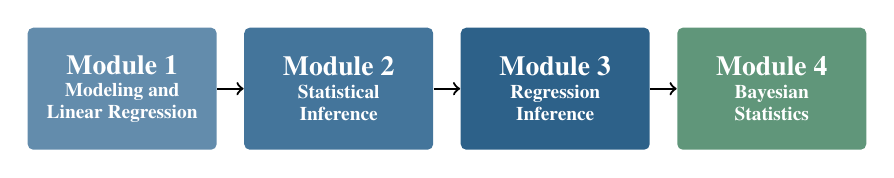
\begin{tikzpicture}[x=1cm,y=1cm]
    \tikzstyle{modulebox}=[draw=none, rounded corners=2pt, minimum width=2.4cm,
      minimum height=1.55cm, text=white, align=center, font=\scriptsize\bfseries]

    \node[modulebox, fill=oiB!75] (m1) at (0,0) {{\normalsize Module 1}\\Modeling and\\Linear Regression};
    \node[modulebox, fill=oiB!90] (m2) at (2.75,0) {{\normalsize Module 2}\\Statistical\\Inference};
    \node[modulebox, fill=oiB!95!black] (m3) at (5.5,0) {{\normalsize Module 3}\\Regression\\Inference};
    \node[modulebox, fill=oiG!90] (m4) at (8.25,0) {{\normalsize Module 4}\\Bayesian\\Statistics};

    \draw[->, line width=0.8pt] (m1.east) -- (m2.west);
    \draw[->, line width=0.8pt] (m2.east) -- (m3.west);
    \draw[->, line width=0.8pt] (m3.east) -- (m4.west);
    \end{tikzpicture}
    \end{center}

    {Building on MA213/DS122...}
	\begin{itemize}
		\item Statistical modeling 
		\item Regression 
		\item Simulation-based inference
		\item Model checking
		\item Bayesian modeling and computation 
	\end{itemize}

\end{frame}

%%%%%%%%%%%%%%%%%%%%%%%%%%%%%%%%%%%
% Textbook

\begin{frame}
	\frametitle{Textbooks (1)}
	\begin{columns}
		\column{0.6\textwidth}
		\begin{minipage}[t]{\linewidth}
		\vspace{0pt}
			\hl{Introduction to Modern Statistics (IMS)}, 2nd Edition \\
			{Mine Cetinkaya-Rundel and Joanna Hardin} \\
						\\
			\webLink{https://www.openintro.org/book/ims/}{https://www.openintro.org/book/ims/} \\
			\\
			Free download as PDF or \$25 for print copy
		\end{minipage}
		\column{0.4\textwidth}
		\begin{minipage}[t]{\linewidth}
		\vspace{0pt}
		\centering
		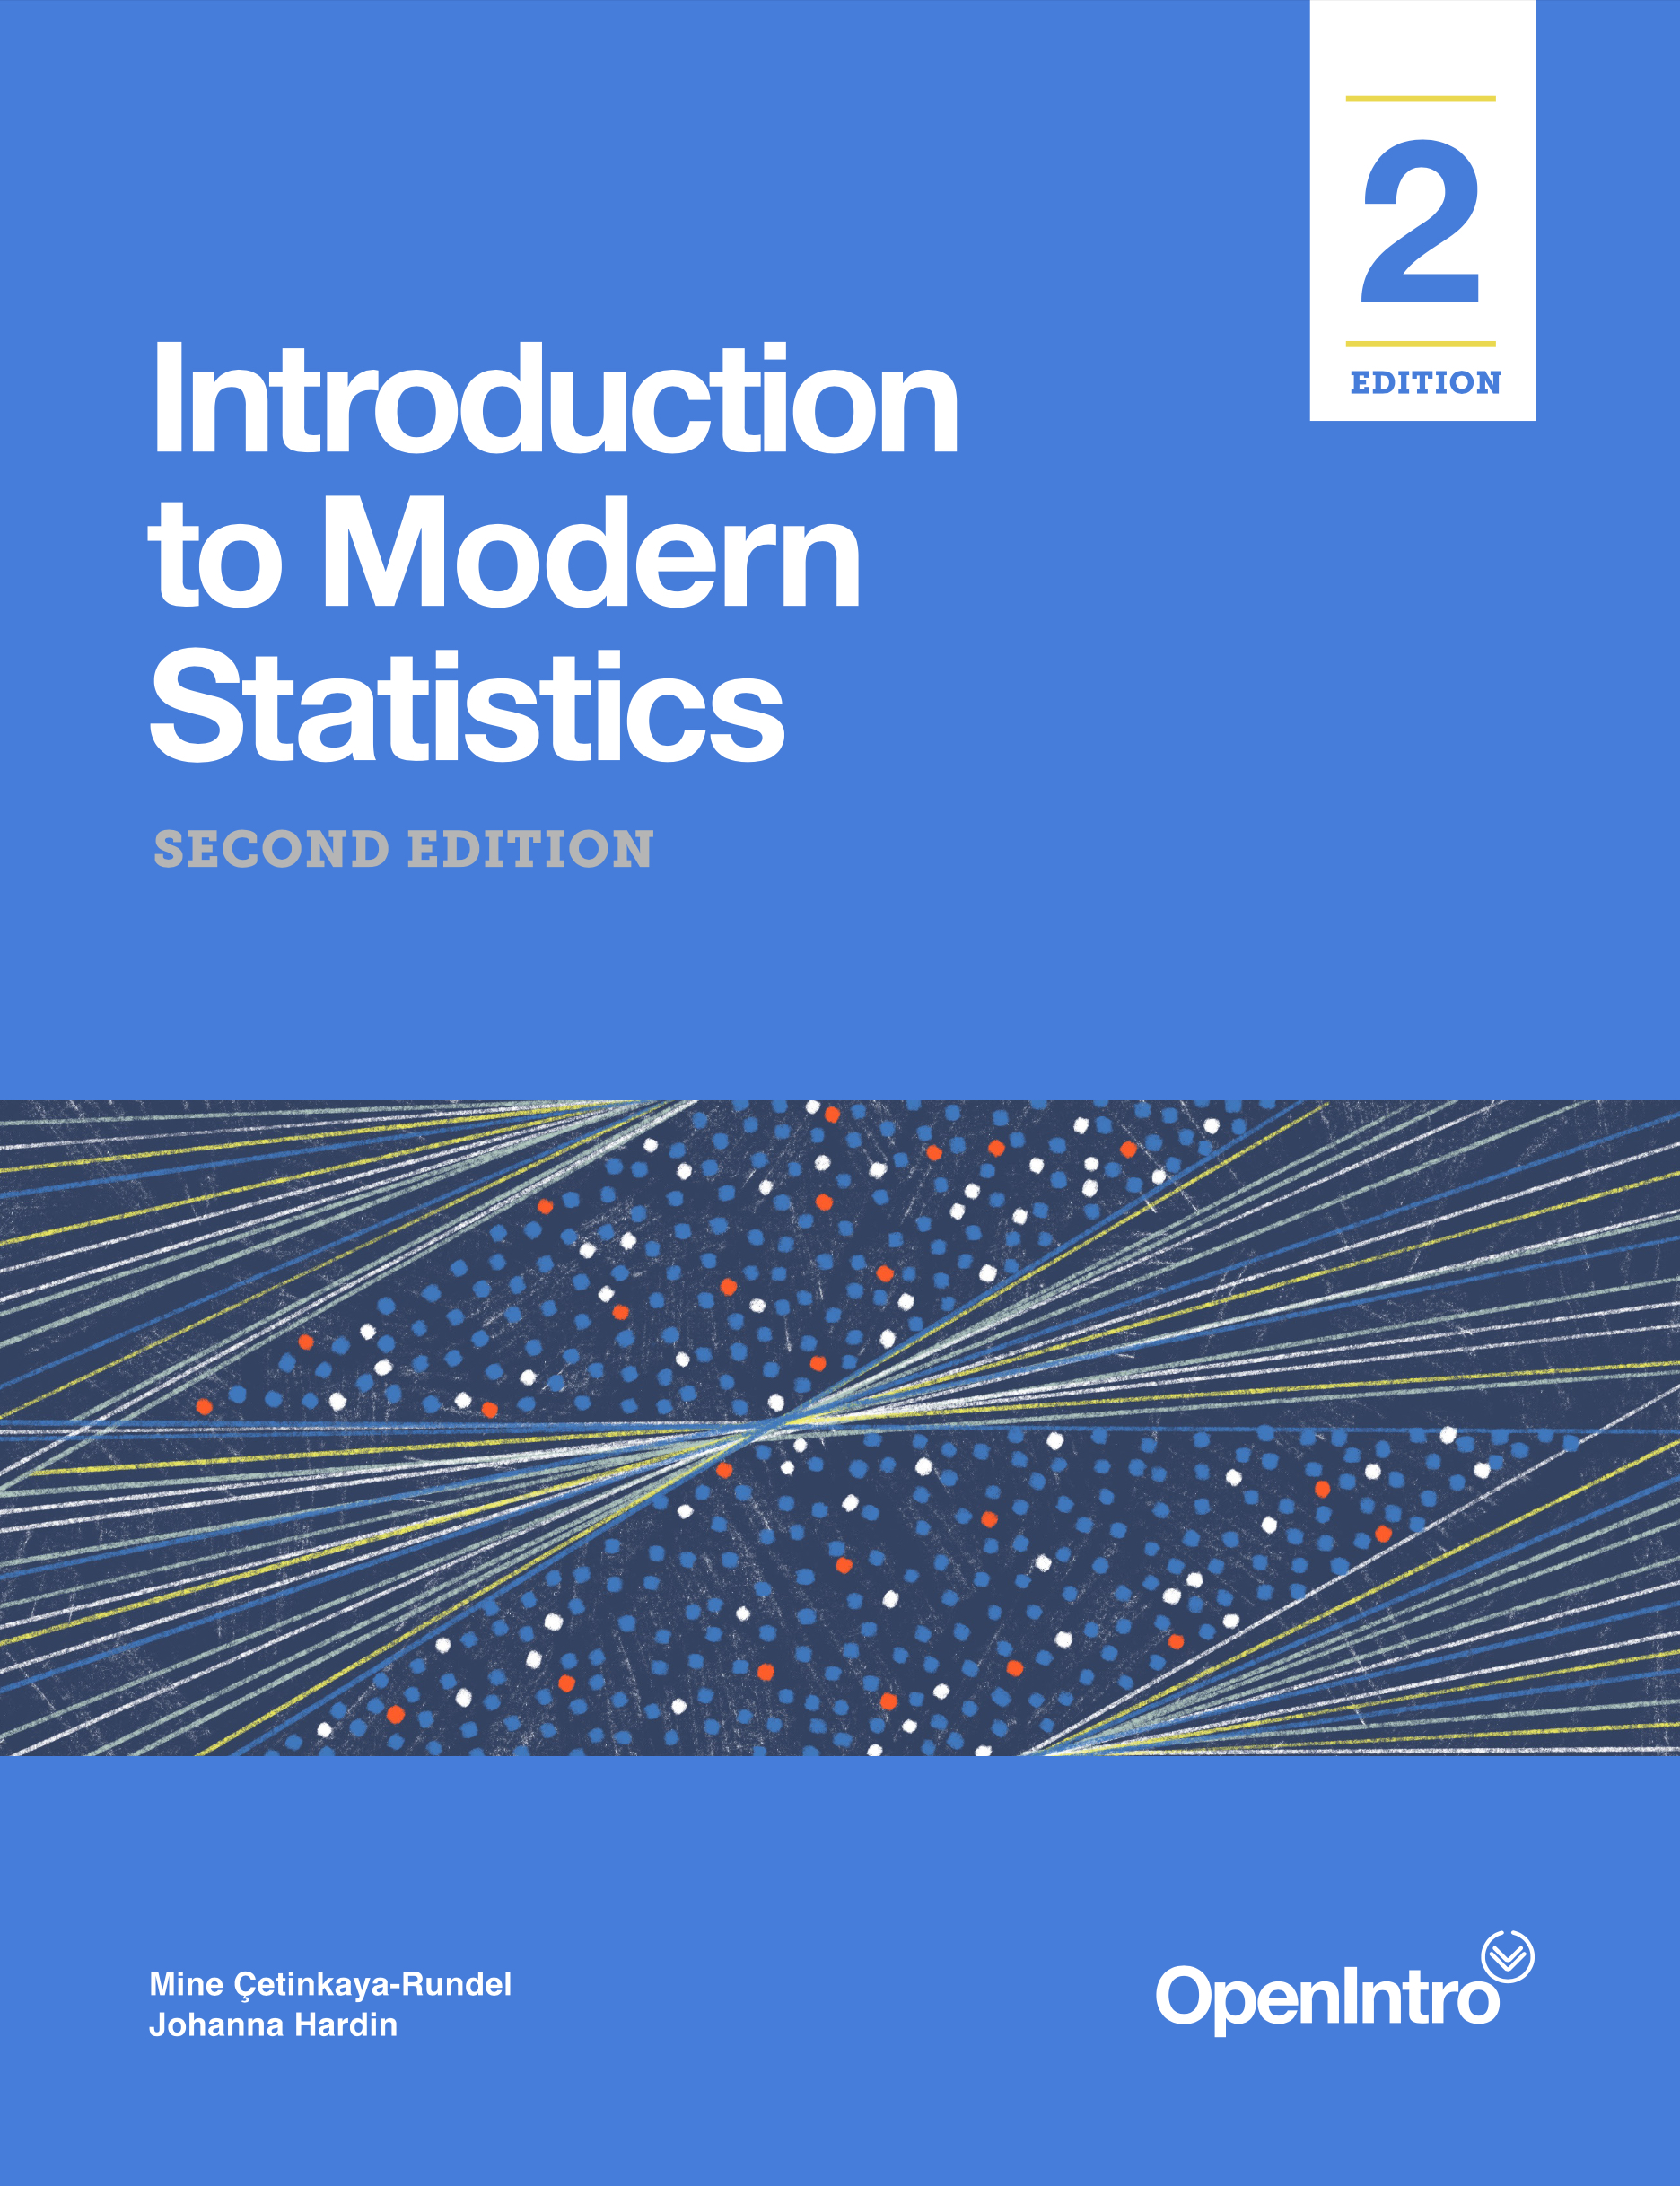
\includegraphics[width=0.9\columnwidth]{figures/IMS2_front_cover.jpeg}
		\end{minipage}
	\end{columns}
\end{frame}


\begin{frame}
	\frametitle{Textbooks (2)}
	\begin{columns}
		\column{0.6\textwidth}
		\begin{minipage}[t]{\linewidth}
		\vspace{0pt}
			\hl{Bayes Rules!} \\
			{Alicia Johnson, Miles Ott, and Mine Dogucu} \\
			\\
			\webLink{https://www.bayesrulesbook.com/}{https://www.bayesrulesbook.com/} \\
			\\
			Free online or get print copy for 20\% using code on website
		\end{minipage}
		\column{0.4\textwidth}
		\begin{minipage}[t]{\linewidth}
		\vspace{0pt}
		\centering
		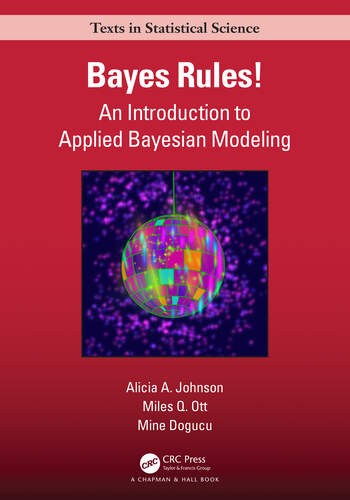
\includegraphics[width=0.9\columnwidth]{figures/bayesrules_cover.jpeg}
		\end{minipage}
	\end{columns}
\end{frame}

%%%%%%%%%%%%%%%%%%%%%%%%%%%%%%%%%%%
% Labs

\begin{frame}
	\frametitle{Labs} 
	\begin{itemize}
		\item \hl{Weekly labs} on Wednesday, starting this week, give you an opportunity to \textbf{apply what you've learned}
		\item \hl{Skills labs}
		\begin{itemize}
			\item Work in pairs
			\item Analyze data and run simulations in R
			\item Post-lab questions to be submitted on Gradescope
		\end{itemize}
		\item \hl{Lab projects}
		\begin{itemize}
			\item Work in groups to explore real data
			\item Project 1: Data analysis video presentation
			\item Project 2: Statistical report
		\end{itemize}
	\end{itemize}
\end{frame}

%%%%%%%%%%%%%%%%%%%%%%%%%%%%%%%%%%%
% Assignments and Grading Structure

\begin{frame}
	\frametitle{Assignments}
	\begin{itemize}
		\item \hl{Written homework}
		\begin{itemize}
			\item About once per week
			\item Graded Satisfactory / Unsatisfactory
		\end{itemize}
		\item \hl{Lecture participation} via in-class activity completion
		\item 4 \hl{Quizzes}
		\begin{itemize}
			\item Cover \hl{22 learning objectives}
			\item 4--6 written problems per quiz, one per learning objective
			\item Each graded Proficient / Approaching Proficiency / Not Yet
			\item Can \hl{qualify} to retake objectives at the end of the semester (details later)
		\end{itemize}
		\item 1 \hl{Final Exam}
		\item 5 \hl{Skills Labs}
		\item 2 \hl{Lab Projects}
	\end{itemize}
\end{frame}

\begin{frame}
	\frametitle{Grading Structure}
	\begin{table}[ht]
	\centering
	\scriptsize
	\renewcommand{\arraystretch}{1.05}
	\begin{tabular}{|l|c|c|c|}
	\hline
	 & \textbf{A} & \textbf{B} & \textbf{C} \\
	\hline
	Quiz objectives (of 22) & 21 passed & 18 passed & 13 passed \\
	\hline
	Final exam & 2 P & 2 AP & 1 AP \\
	\hline
	Lab projects & 2 satisfactory & 2 satisfactory & 2 satisfactory \\
	\hline
	Skills labs (of 5) & 5 passed & 4 passed & 3 passed \\
	\hline
	Written homework & $\le$1 not passed & $\le$3 not passed & $\le$5 not passed \\
	\hline
	Lecture worksheets & $\le$3 missed & $\le$5 missed & $\le$9 missed \\
	\hline
	Labs & $\le$2 missed & $\le$3 missed & $\le$4 missed \\
	\hline
	\end{tabular}
	\end{table}
	\vspace{-0.4em}
	{\scriptsize \hspace{3em} P = Proficient, AP = Approaching Proficiency (see Quizzes).}

	\hl{Additional factors:}
	\begin{itemize}\itemsep=1pt
		\item Every row's requirement must be met for a given grade.
		\item An ``unsatisfactory'' project drops your grade two-thirds of a letter (B $\to$ C+).
		\item Lectures missed with permission do not count as missed.
	\end{itemize}
\end{frame}

%%%%%%%%%%%%%%%%%%%%%%%%%%%%%%%%%%%
% Learning Objectives



%%%%%%%%%%%%%%%%%%%%%%%%%%%%%%%%%%%

\begin{frame}
	\frametitle{Class Policies} 
	\begin{itemize}
		\item \hl{Attendance and participation:}
		\begin{itemize}
			\item Attend all lectures, labs, and discussions.
			\item In-class activities count toward your grade.
			\item Email the relevant instructor or your discussion TF if you must miss a session.
		\end{itemize}
		\item \hl{Academic integrity:}
		\begin{itemize}
			\item All work must be your own.
			\item Collaboration is allowed on homework and labs/projects, \textbf{not on quizzes}.
		\end{itemize}
		\item \hl{Use of Generative AI tools (e.g., ChatGPT, Claude, CoPilot):}
		\begin{itemize}
			\item Quizzes: \textbf{not allowed}.
			\item Homework: use at your own discretion.
			\item Labs/Projects: allowed for \textbf{specific uses}.
		\end{itemize}
	\end{itemize}

	\vspace{0.3em}
	{\footnotesize See the Syllabus for the full integrity and GenAI policies.}
\end{frame}

%%%%%%%%%%%%%%%%%%%%%%%%%%%%%%%%%%%
% Calendar
\begin{frame}
	\frametitle{Overview: Weekly Cadence} 
	\begin{itemize}
		\item \hl{Monday:} 
			\begin{itemize}
				\item Discussion sections meet
			\end{itemize}
		\item \hl{Tuesday:} 
			\begin{itemize}
				\item Lecture
				\item Lab deliverable due
				\item Problem sets due at noon 
			\end{itemize}
		\item \hl{Wednesday:} 
			\begin{itemize}
				\item Lab sections meet
			\end{itemize}
		\item \hl{Thursdays:} 
			\begin{itemize}
				\item Lecture
			\end{itemize}
		\item \hl{Friday:} Nothing :-)
	\end{itemize}
\end{frame}
%%%%%%%%%%%%%%%%%%%%%%%%%%%%%%%%%%%

%%%%%%%%%%%%%%%%%%%%%%%%%%%%%%%%%%%%
\section{Statistics and Probability Review}

%%%%%%%%%%%%%%%%%%%%%%%%%%%%%%%%%%%%%%%%%%%%%%%%%%%%%%%%%%%%%%%%%%%%%%%%
% Lecture goals
\begin{frame}
    \frametitle{Lecture Objectives}
    \goals{%
    \begin{itemize}
    \item describe the big picture of statistics: producing data, describing data, and drawing inferences;
    \item explain what a random process is and why we model processes as random;
    \item interpret a probability and distinguish the frequentist and Bayesian interpretations.
    \end{itemize}}
\end{frame}
%%%%%%%%%%%%%%%%%%%%%%%%%%%%%%%%%%%%

%%%%%%%%%%%%%%%%%%%%%%%%%%%%%%%%%%%
% Big picture of statistics 
% https://stats.libretexts.org/Bookshelves/Applied_Statistics/Biostatistics_-_Open_Learning_Textbook/Preliminaries/The_Big_Picture
% https://creativecommons.org/licenses/by-nc-sa/4.0/

%%%%%%%%%%%%%%%%%%%%%%%%%%%%%%%%%%%%%%%%%%%%%%%%%%%%%%%%%%%%%%%%%%%%%%%%
\begin{frame}
    \frametitle{Big Picture of Statistics}
    \begin{center}
        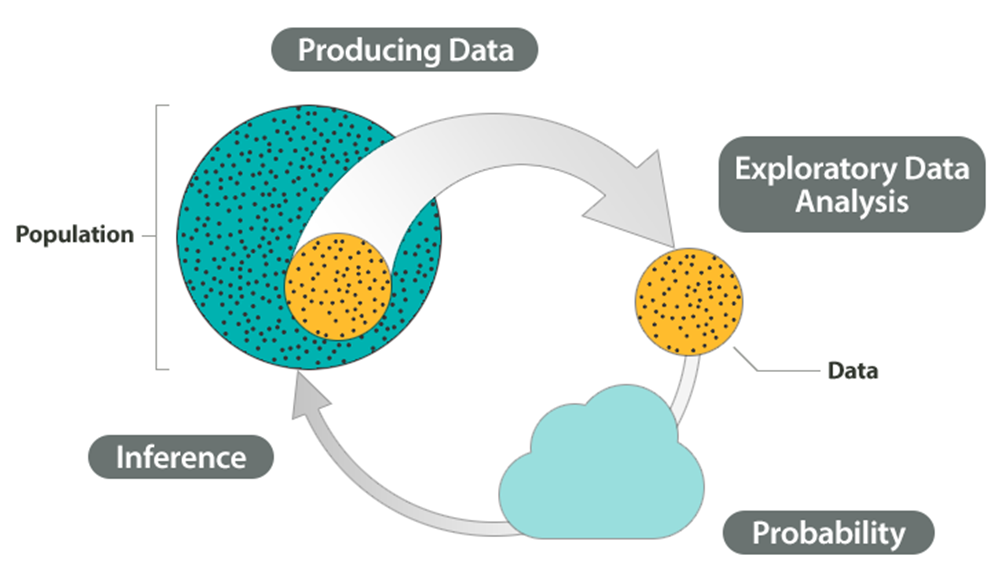
\includegraphics[width=0.95\textwidth]{figures/BigPicture.png}
    \end{center}
    \vspace{0.5em}
    {\footnotesize
    Credit: \href{https://stats.libretexts.org/Bookshelves/Applied_Statistics/Biostatistics_-_Open_Learning_Textbook/Preliminaries/The_Big_Picture}{LibreTexts}, 
    licensed under \href{https://creativecommons.org/licenses/by-nc-sa/4.0/}{CC BY-NC-SA 4.0}.}
\end{frame}


%%%%%%%%%%%%%%%%%%%%%%%%%%%%%%%%%%%%%%%%%%%%%%%%%%%%%%%%%%%%%%%%%%%%%%%%
\begin{frame}
    \frametitle{Big Picture of Statistics: Obtaining and Describing Data}
    \begin{center}
        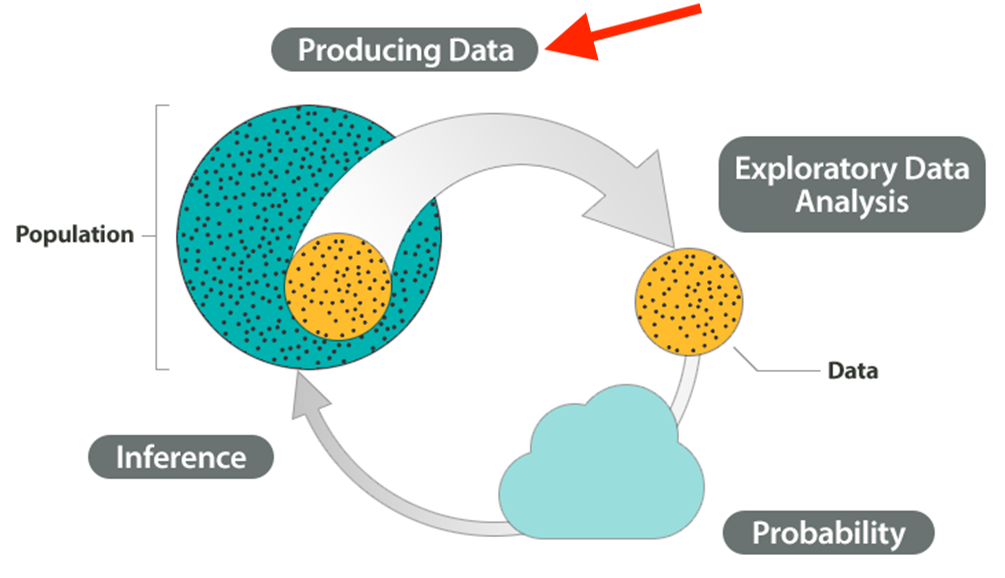
\includegraphics[width=0.95\textwidth]{figures/BigPicture-producing-data.png}
    \end{center}
    \vspace{0.5em}
    {\footnotesize
    Credit: \href{https://stats.libretexts.org/Bookshelves/Applied_Statistics/Biostatistics_-_Open_Learning_Textbook/Preliminaries/The_Big_Picture}{LibreTexts}, 
    licensed under \href{https://creativecommons.org/licenses/by-nc-sa/4.0/}{CC BY-NC-SA 4.0}.}
\end{frame}

\subsection{Random Process and Probability}
%%%%%%%%%%%%%%%%%%%%%%%%%%%%%%%%%%%%%%%%%%%%%%%%%%%%%%%%%%%%%%%%%%%%%%%%
\begin{frame}
    \frametitle{Random Processes}
    A \hl{random process} produces outcomes we know are \emph{possible}, but cannot predict.

    \vspace{0.15cm}
    Common types:
    \begin{itemize}\itemsep=3pt
        \item \textbf{Chance experiment:} a repeatable action. A coin lands heads or tails; a die shows 1--6.
        \item \textbf{Random sampling:} drawing individuals at random. Each sample of 100 students holds different people.
        \item \textbf{Real-world observation:} an outcome not settled until it happens. Whether a flight arrives on time.
    \end{itemize}

    \vspace{0.15cm}
    We can model a process \hl{as if} it were random when it behaves that way.
\end{frame}

%%%%%%%%%%%%%%%%%%%%%%%%%%%%%%%%%%%%%%%%%%%%%%%%%%%%%%%%%%%%%%%%%%%%%%%%
\begin{frame}{Outcomes and Events}
    For a random process:
    \begin{itemize}
        \item An \hl{outcome} is a single possible result.
        \item The \hl{sample space} is the set of all possible outcomes.
        \item An \hl{event} is a collection of outcomes we care about --- a subset of the sample space.
    \end{itemize}

    \vspace{0.25cm}
    \begin{center}
    \footnotesize
    \renewcommand{\arraystretch}{1.25}
    \begin{tabular}{lll}
    \hline
    Random process & An outcome & An event \\
    \hline
    Flip 3 coins & heads, tails, tails & ``lands on heads twice'' \\
    Sample 100 students & one particular set of 100 & ``at least 60 are seniors'' \\
    A scheduled flight & arrives 5 min early & ``the flight arrives late'' \\
    A blood-pressure reading & $138$ mmHg & ``reading above $140$'' \\
    \hline
    \end{tabular}
    \end{center}
\end{frame}

%%%%%%%%%%%%%%%%%%%%%%%%%%%%%%%%%%%%%%%%%%%%%%%%%%%%%%%%%%%%%%%%%%%%%%%%
\begin{frame}{Probability}
    The \hl{probability} of an event $A$ measures how likely it is, on a scale from $0$ to $1$:
    \[ 0 \le P(A) \le 1, \qquad P(A)=0:\ \text{impossible}, \quad P(A)=1:\ \text{certain}. \]
    For a fair coin $P(\text{heads}) = 0.5$; for a flight we might have $P(\text{delayed}) = 0.2$.

    \begin{itemize}
      \item \textbf{Frequentist:} the long-run proportion of replications in which $A$ occurs.
      \item \textbf{Bayesian:} the degree of belief that $A$ will occur.
    \end{itemize}

    \vspace{0.15cm}
    We will use both perspectives in this course.
\end{frame}


%%%%%%%%%%%%%%%%%%%%%%%%%%%%%%%%%%%%%%%%%%%%%%%%%%%%%%%%%%%%%%%%%%%%%%%%
\begin{frame}{Basic Probability Rules}
\begin{columns}[T]
\column{0.54\textwidth}
    \formula{Rules}{%
    \begin{itemize}
    \item \textbf{Complement:} $P(A^c) = 1 - P(A)$.
    \item \textbf{Addition:} \\ $P(A \cup B) = P(A) + P(B) - P(A \cap B)$.
    \item \textbf{If $A$, $B$ independent:} \\ $P(A \cap B) = P(A)\,P(B)$.
    \end{itemize}}

\column{0.46\textwidth}
\centering
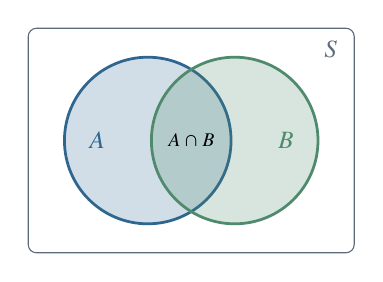
\begin{tikzpicture}[scale=0.92]
    % sample space
    \draw[rounded corners=3pt, draw=ccGray] (-2.25,-1.55) rectangle (2.25,1.55);
    \node[ccGray, font=\small] at (1.95,1.25) {$S$};
    % overlapping events (double overlap darkens the intersection)
    \draw[ccBlue,  fill=ccBlue,  fill opacity=0.22, line width=1pt] (-0.6,0) circle (1.15);
    \draw[ccGreen, fill=ccGreen, fill opacity=0.22, line width=1pt] ( 0.6,0) circle (1.15);
    \node[ccBlue,  font=\small] at (-1.3,0) {$A$};
    \node[ccGreen, font=\small] at ( 1.3,0) {$B$};
    \node[font=\scriptsize] at (0,0) {$A \cap B$};
\end{tikzpicture}

\vspace{0.4em}
{\footnotesize The overlap $A \cap B$ is counted in \emph{both} $P(A)$ and $P(B)$, so the ``or'' rule subtracts it once.}
\end{columns}
\end{frame}



%%%%%%%%%%%%%%%%%%%%%%%%%%%%%%%%%%%%

%%%%%%%%%%%%%%%%%%%%%%%%%%%%%%%%%%%%%%%%%%%%%%%%%%%%%%%%%%%%%%%%%%%%%%%%
\begin{frame}{Activity: Interpreting a Probability}
\activity[-- Interpreting a probability]{%
A weather model gives $P(\text{rain tomorrow}) = 0.30$.
\begin{enumerate}
  \item Out of 100 days with similar conditions, about how many would you expect to have rain?
  \item If tomorrow and the next day have similar, \emph{independent} conditions, find $P(\text{no rain on either day})$.
  \item If it does not rain tomorrow, does that mean the model was wrong? Explain briefly.
\end{enumerate}}

\solnbox{1.~About $30$ days. \quad 2.~$0.7 \times 0.7 = 0.49$. \quad 3.~No --- a 30\% event failing to occur is expected and does not contradict the model.}
\end{frame}


%%%%%%%%%%%%%%%%%%%%%%%%%%%%%%%%%%%
% not sure if we want to include this
%%%%%%%%%%%%%%%%%%%%%%%%%%%%%%%%%%%%%%%%%%%%%%%%%%%%%%%%%%%%%%%%%%%%%%%%
\begin{frame}{Law of Large Numbers: proportions}
For an event with true probability $p$, let $\hat{p}_n$ be the \hl{observed proportion} of times it occurs in $n$ trials. Then $\hat{p}_n \to p$ as $n$ grows.

\begin{center}
    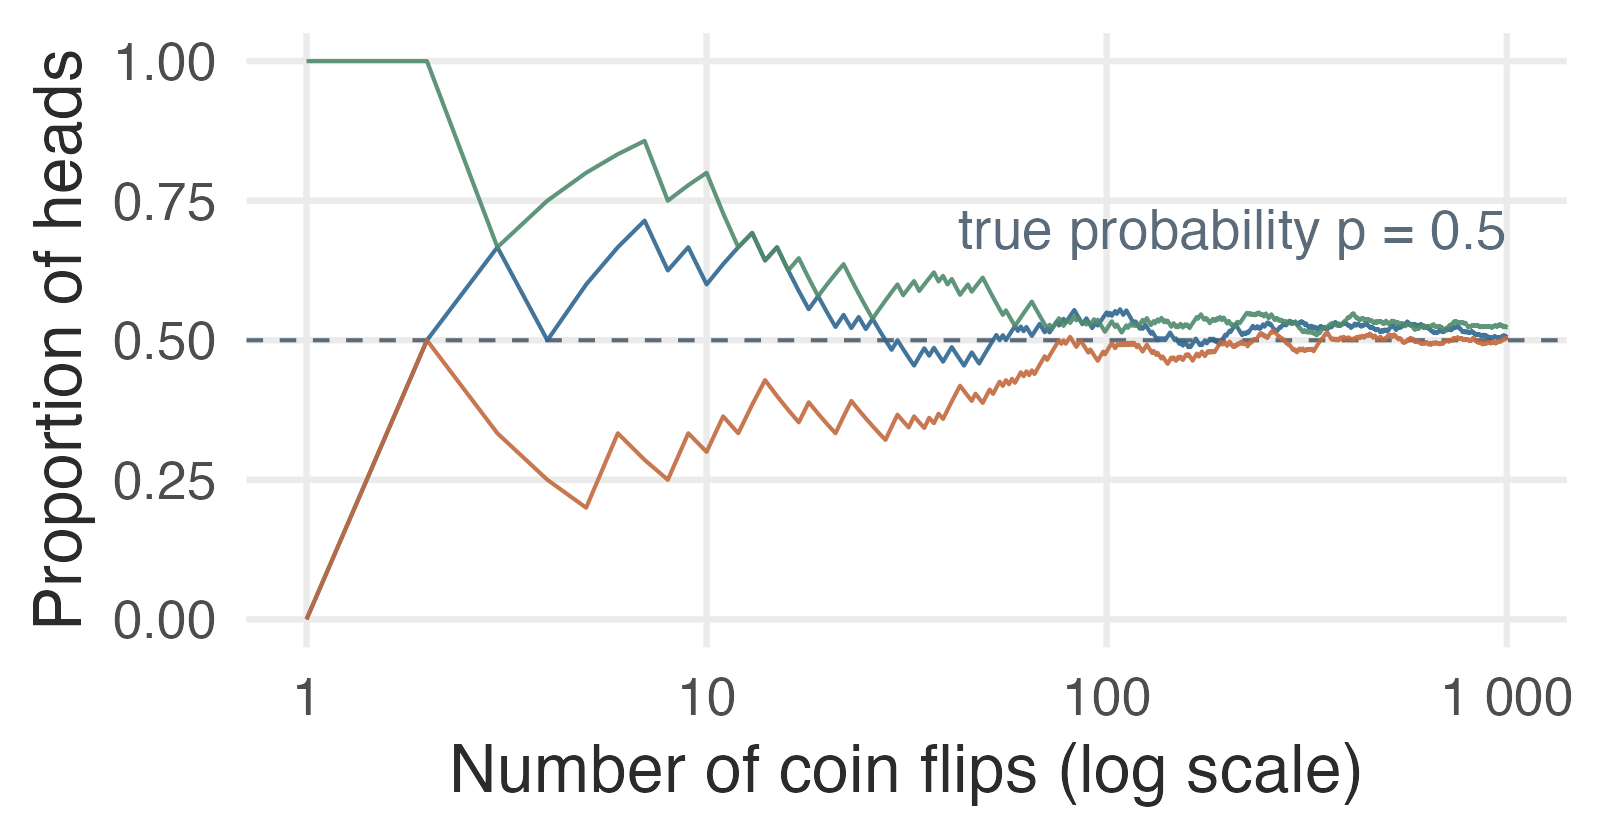
\includegraphics[width=0.6\textwidth]{figures/lln_running_proportion.png}
\end{center}

\vspace{-0.25cm}
{\footnotesize Three runs of a fair coin ($p=0.5$): each running proportion of heads settles toward $p$ as the number of flips grows.}
\end{frame}

%%%%%%%%%%%%%%%%%%%%%%%%%%%%%%%%%%%%%%%%%%%%%%%%%%%%%%%%%%%%%%%%%%%%%%%%
\begin{frame}{Law of Large Numbers: means}
The same holds for averages. For observations with true (population) mean $\mu$, let $\bar{x}_n$ be the \hl{sample mean} of $n$ observations. Then $\bar{x}_n \to \mu$ as $n$ grows.

\begin{center}
    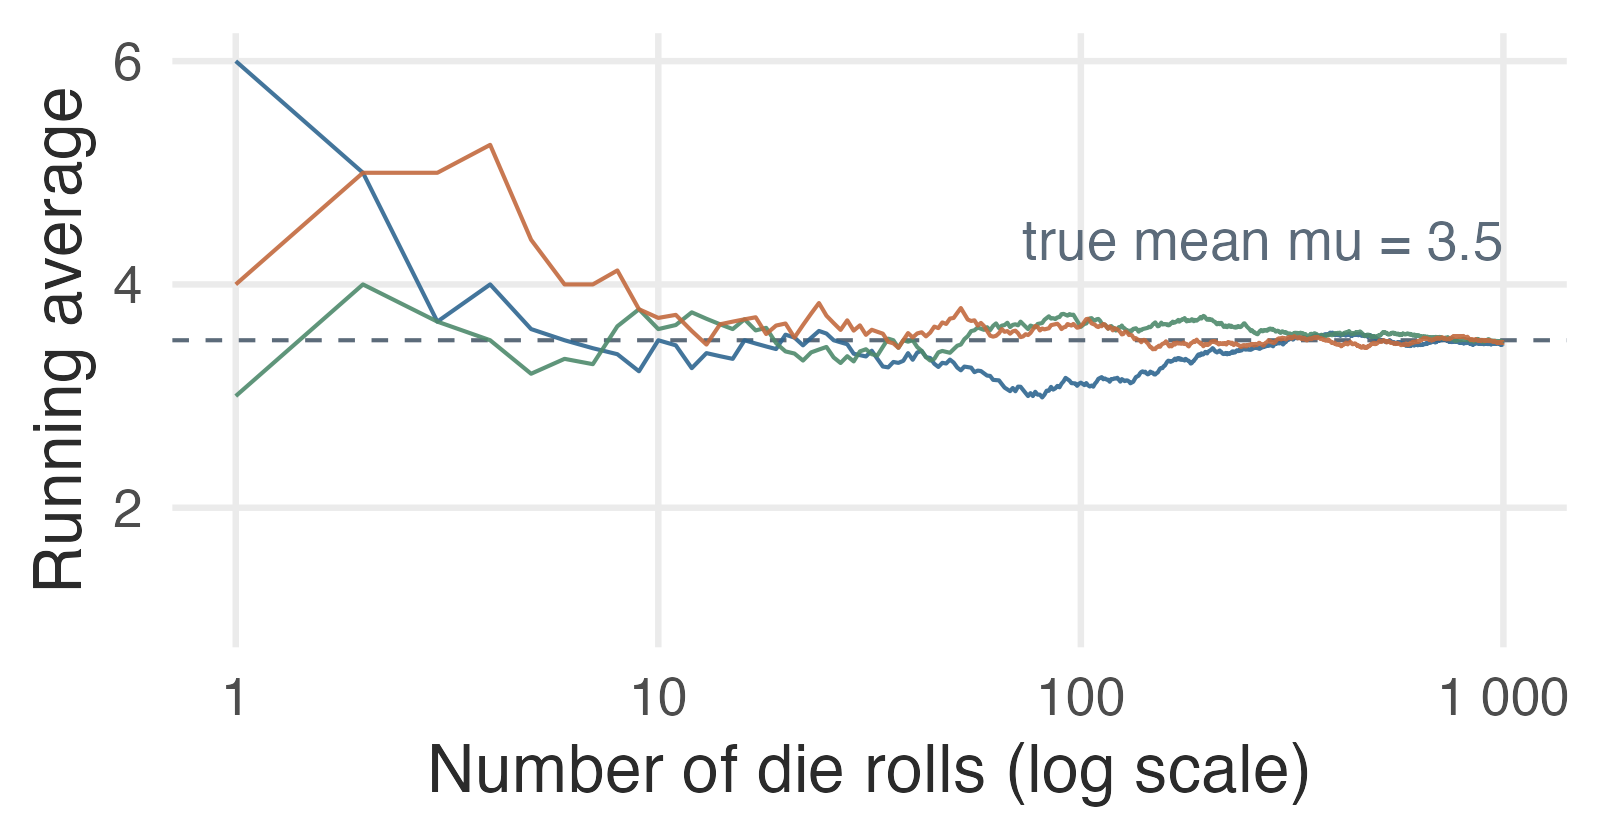
\includegraphics[width=0.6\textwidth]{figures/lln_running_mean.png}
\end{center}

\vspace{-0.25cm}
{\footnotesize Three runs of rolling a fair die ($\mu = 3.5$): each running average settles toward $\mu$. \hl{Larger samples give more stable estimates than small ones.}}
\end{frame}



%%%%%%%%%%%%%%%%%%%%%%%%%%%%%%%%%%%

\subsection{Data-Generating, Inference}

%%%%%%%%%%%%%%%%%%%%%%%%%%%%%%%%%%%

%%%%%%%%%%%%%%%%%%%%%%%%%%%%%%%%%%%%%%%%%%%%%%%%%%%%%%%%%%%%%%%%%%%%%%%%
\begin{frame}{Data-Generating Processes}
\keyidea[-- Data-generating process]{A real-world, random process that produces the data we observe.}

\begin{center}
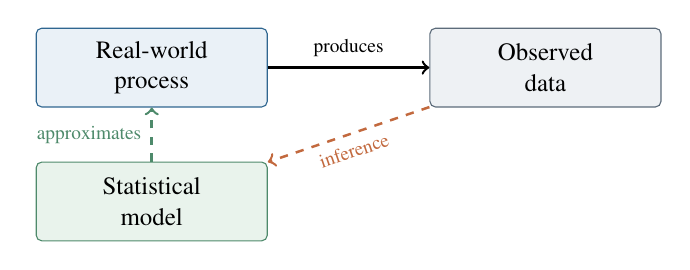
\begin{tikzpicture}[x=1cm,y=1cm,
    box/.style={draw, rounded corners=2pt, align=center, font=\small,
                minimum height=1cm, text width=2.7cm}]
    \node[box, fill=ccBlueBg,  draw=ccBlue]  (proc)  at (0,0)    {Real-world\\process};
    \node[box, fill=ccGrayBg,  draw=ccGray]  (data)  at (5,0)    {Observed\\data};
    \node[box, fill=ccGreenBg, draw=ccGreen] (model) at (0,-1.7) {Statistical\\model};
    \draw[->, line width=0.9pt] (proc) -- node[above, font=\scriptsize]{produces} (data);
    \draw[->, line width=0.9pt, dashed, ccGreen] (model) -- node[left, font=\scriptsize]{approximates} (proc);
    \draw[->, line width=0.9pt, dashed, ccTerra] (data) -- node[below, sloped, font=\scriptsize]{inference} (model);
\end{tikzpicture}
\end{center}

A \hl{statistical model} is a simplified description of that process. Using \green{data} to learn about the model is \green{statistical inference}.
\end{frame}



%%%%%%%%%%%%%%%%%%%%%%%%%%%%%%%%%%%%%%%%%%%%%%%%%%%%%%%%%%%%%%%%%%%%%%%%
\begin{frame}
\frametitle{Goals of statistical inference}

Statistical inference can serve many different goals.

\begin{itemize}
\item \textbf{Description:} What patterns are in this dataset?
\item \textbf{Estimation:} What is an unknown parameter value?
\item \textbf{Testing:} Is the observed pattern surprising under a baseline or assumed model?
\item \textbf{Prediction:} Can we predict future or unobserved outcomes?
\item \textbf{Causation:} What would change under an intervention such as a medical treatment? 
\end{itemize}

\end{frame}




%%%%%%%%%%%%%%%%%%%%%%%%%%%%%%%%%%%%%%%%%%%%%%%%%%%%%%%%%%%%%%%%%%%%%%%%
\begin{frame}
\frametitle{Two primary types of data collection}

\begin{itemize}

\item \hl{Observational studies:} Collect data in a way that does not directly interfere with how the data arise (e.g., surveys).
\begin{itemize}
\item We observe data without assigning treatments or interventions.
\item Useful for describing patterns, prediction, and sometimes causal questions
\item Causal claims require additional assumptions
\end{itemize}

\pause

\item \hl{Experiment:} Researchers randomly assign subjects to various treatments in order to establish causal connections between the explanatory and response variables.
\begin{itemize}
\item Researchers assign treatments, ideally at random.
\item Randomization helps balance confounders between groups.
\item Causal conclusions still require assumptions, including compliance, valid measurement, and relevance to the target setting.
\end{itemize}


\end{itemize}

\end{frame}






%%%%%%%%%%%%%%%%%%%%%%%%%%%%%%%%%%%%%%%%%%%%%%%%%%%%%%%%%%%%%%%%%%%%%%%%
\begin{frame}{Parameter, Statistic, and Point Estimate}

\begin{itemize}
  \item A \textbf{parameter} is a fixed but usually unknown quantity determined by the data-generating process.
  \item A \textbf{statistic} is a quantity computed from observed data.
  \item A \textbf{point estimate} uses a statistic to estimate a parameter.
\end{itemize}

\vspace{0.4em}
We put these to work in a running example we return to through the rest of the section.

\end{frame}

%%%%%%%%%%%%%%%%%%%%%%%%%%%%%%%%%%%%%%%%%%%%%%%%%%%%%%%%%%%%%%%%%%%%%%%%
\begin{frame}{A running example}
\examplehead{Blood-pressure study}

A clinical study gives patients a new blood-pressure drug and records the \hl{reduction in systolic blood pressure} after eight weeks.

\begin{itemize}
\item \hl{Question:} what is the mean reduction for the target population of patients?
\item \hl{Data:} the reductions measured for a random sample of $100$ patients.
\end{itemize}

\vspace{0.3em}
The \textbf{parameter} is $\mu$ = the true mean reduction in the population; the \textbf{statistic} is $\bar{x}$ = the mean reduction in our sample. So $\bar{x}$ is a \hl{point estimate} of $\mu$.
\end{frame}



%%%%%%%%%%%%%%%%%%%%%%%%%%%%%%%%%%%%%%%%%%%%%%%%%%%%%%%%%%%%%%%%%%%%%%%%
\begin{frame}
\frametitle{Sampling variability}
\examplehead{Blood-pressure study}

Repeating the study with different random samples, the sample mean changes:
\[
\bar{x}_1 = 7.8,\qquad \bar{x}_2 = 5.9,\qquad \bar{x}_3 = 6.6
\]
A \textbf{parameter} ($\mu$) is fixed; a \textbf{statistic} ($\bar{x}$) varies from sample to sample. This \hl{sampling variability} is one reason we need statistical inference.

\end{frame}


%%%%%%%%%%%%%%%%%%%%%%%%%%%%%%%%%%%%%%%%%%%%%%%%%%%%%%%%%%%%%%%%%%%%%%%%
\begin{frame}
\frametitle{Sampling distribution}
\examplehead{Blood-pressure study}

Repeatedly take a random sample of patients and compute its mean reduction $\bar{x}$. The distribution of those means is the \hl{sampling distribution} of $\bar{x}$.

\vspace{0.1em}
\centering
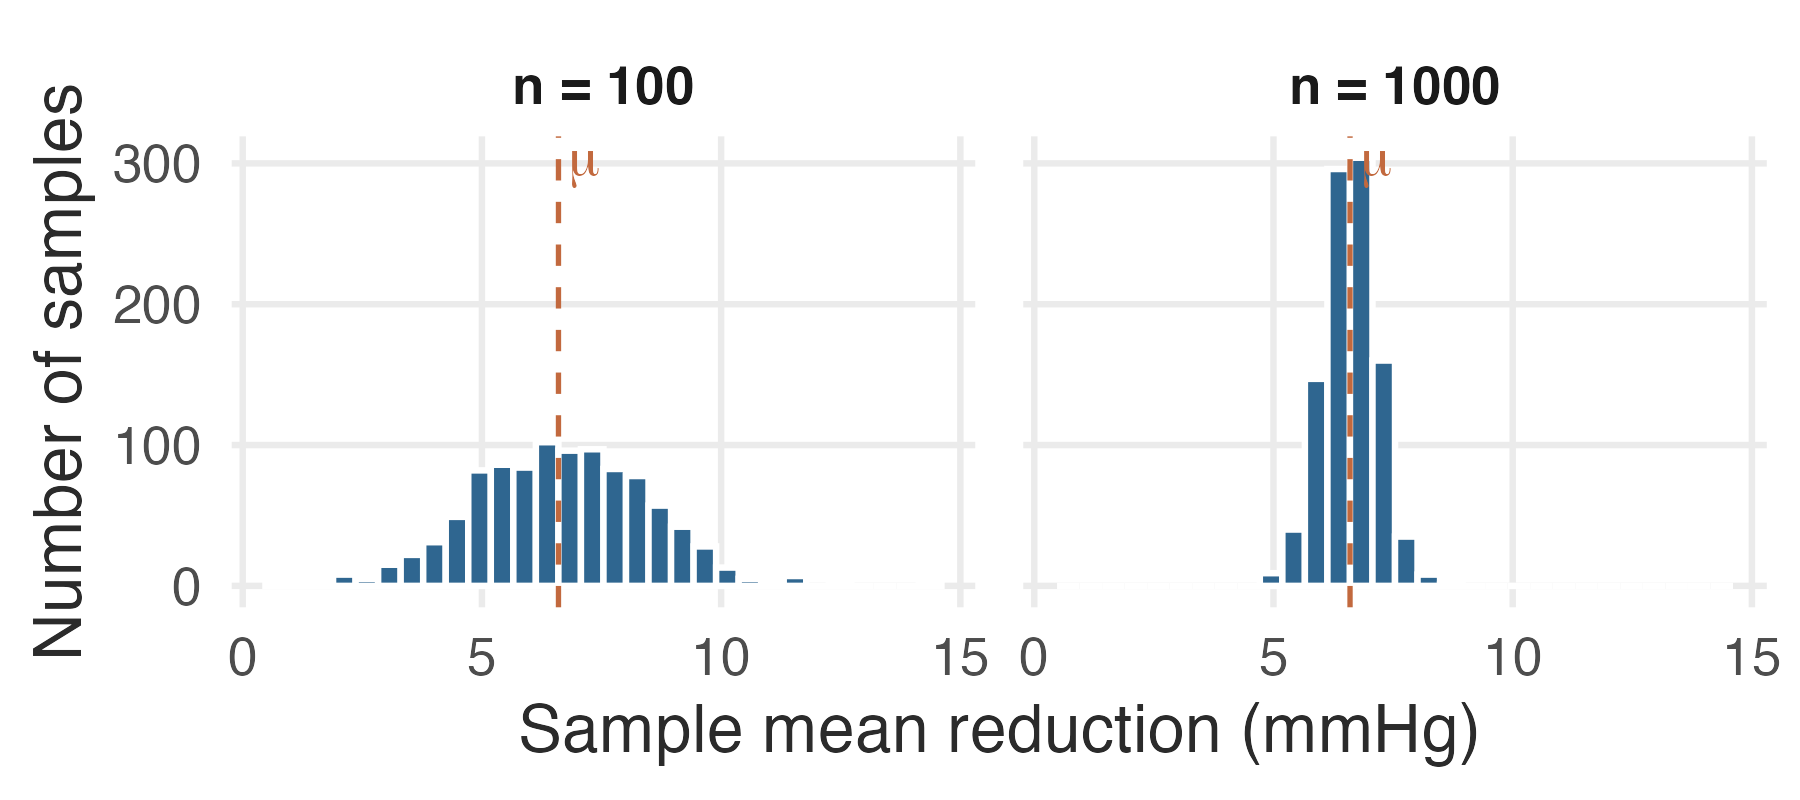
\includegraphics[width=0.86\textwidth]{figures/sampling_distribution_means.png}

\end{frame}

%%%%%%%%%%%%%%%%%%%%%%%%%%%%%%%%%%%%%%%%%%%%%%%%%%%%%%%%%%%%%%%%%%%%%%%%
\begin{frame}
\frametitle{Activity: parameter, statistic, or inference?}
\examplehead{Blood-pressure study}
\begin{center}
\footnotesize
\renewcommand{\arraystretch}{0.9}
\begin{tabular}{lcc}
\hline
Group & Number of patients & Mean reduction in systolic BP\\
\hline
Under 50 & 38 & 5.8 mmHg\\
50 or older & 62 & 7.1 mmHg\\
All sampled patients & 100 & 6.6 mmHg\\
\hline
\end{tabular}
\end{center}
\vspace{-0.7em}
\activity[-- Classify each statement]{\small
Is each statement referencing a \hl{parameter}, a \hl{statistic}, or an \hl{inference}?
\vspace{-1.5em}
\begin{enumerate}
\item The 100 sampled patients averaged a 6.6 mmHg reduction.
\item The true mean reduction for all similar patients is unknown.
\item We estimate the true mean reduction at about 6.6 mmHg.
\item The true mean reduction for patients 50 or older is 7.4 mmHg.
\end{enumerate}}
\end{frame}

%%%%%%%%%%%%%%%%%%%%%%%%%%%%%%%%%%%%%%%%%%%%%%%%%%%%%%%%%%%%%%%%%%%%%%%%
\begin{frame}
\frametitle{Activity: parameter, statistic, or inference? --- solution}
\solnbox{%
\begin{enumerate}
\item \textbf{Statistic} --- computed from the observed sample.
\item \textbf{Parameter} --- a fixed, unknown quantity about the population.
\item \textbf{Inference} --- using a statistic to estimate a parameter.
\item \textbf{Parameter} --- $\mu_{50+}$ is a quantity about the population.
\end{enumerate}}
\end{frame}



%%%%%%%%%%%%%%%%%%%%%%%%%%%%%%%%%%%

% Final announcements 
%% !TEX root =  Lecture1.tex

%%%%%%%%%%%%%%%%%%%%%%%%%%%%%%%%%%%%
% Recap/Agenda
%%%%%%%%%%%%%%%%%%%%%%%%%%%%%%%%%%%%
\begin{frame}
\frametitle{Lecture Overview}
\todo[inline]{TODO: update}
    \begin{itemize}
        \item \hl{This time:} course overview, then a review of key concepts --- random processes and probability, data-generating and sampling distributions, and the goals of inference.
        \item \hl{Homework for Thursday:} 
        \item \hl{Reading (optional):} IMS Chapters 1--3.
        \item \hl{Announcements:}
        \begin{itemize}
            \item Labs start \hl{tomorrow} (Wednesday); discussions start Monday.
            \item Email the instructor for any registration issues.
        \end{itemize}
    \end{itemize}
\end{frame}


%%%%%%%%%%%%%%%%%%%%%%%%%%%%%%%%%%%

%%%%%%%%%%%%%%%%%%%%%%%%%%%%%%%%%%%%
% End document
%%%%%%%%%%%%%%%%%%%%%%%%%%%%%%%%%%%%

\end{document}
